
\pagestyle{fancy} \frenchspacing
\lhead{StageControl - automatisierte Steuerung von Ton- und Lichtanlagen (2024/2025)}
\renewcommand{\chaptermark}[1]{\markboth{#1}{}}

\renewcommand{\textfraction}{0}
\renewcommand{\floatpagefraction}{0.999}
\renewcommand{\topfraction}{0.7}
\renewcommand{\bottomfraction}{0.999}
\lfoot{}

\chapter{Grundlagen und Methoden}

\section{Etablierte Lösungsansätze}
Das Kapitel listet etablierte Lösungsansätze zur Standortermittlung einer Person auf einer Bühne und erklärt diese genauer. Ebenso wie Vor- und Nachteile anhand eines Beispieles.

\subsection{Ausgangsituation des Praxisbeispiels}

Man befindet sich auf der Bühne in der Stadthalle in Ybbs. Folgende Informationen sind wichtig.
\begin{itemize}
	\item \textbf{Gerät zur Standortermittlung: } Android Smartphone
	\item \textbf{Koordinaten der Position: } TBD  
\end{itemize}

\subsection{Manuelle Steuerung}
Eine Person steht auf der Bühne der XY. Eine Möglichkeit die Steuerung der Ton- und Lichtanlagen ist diese für das Event vorher zu programmieren oder manuell während der Show zu steuern. Nun fragt sich die Person: "Wie kann ich diese Ton- und Lichtanlagen steuern?" Die Antworten folgen:

\begin{itemize}
	\item "Manuelle Steuerung der Tonanlage"
	\item "Vorprogrammierung der Lichtanlage"
\end{itemize}

An den erlangten Antworten, kann man erkennen, dass es noch keine automatisierte Lösung für das Problem gibt. Die Genauigkeit der Standortermittlung, die für die automatisierte Steuerung der Anlagen notwendig ist, kann in folgende Stufen eingeteilt werden: 

\begin{itemize}
	\item \textbf{Stufe 1: }Standort auf Bühne eingeschränkt
	\item \textbf{Stufe 2: }Standort auf Länge und Breite der Bühne eingeschränkt
	\item \textbf{Stufe 3: }Standort auf bestimmten Punkt auf der Bühne eingeschränkt
\end{itemize}

\section{Hardwareproduktion }
Im Fall von StageControl versteht man unter Hardware nicht nur Computerkomponenten, sondern auch eine eigens hergestellte Konstruktion, die das Funktionieren der Software bzw. der angesteuerten Hardwarekomponenten erst möglich macht.

\subsection{Gerüst}
 So benötigen wir eine Konstruktion/Gerüst, welche uns ermöglicht, die Servomotoren, die Schieberegler steuern, die die Bewegung des Künstlers bzw. der Künstlerin in mechanische Bewegung übertragen, um den gewünschten Stereoeffekt erzeugen. Dies soll möglichst einfach oberhalb des benötigten Mischpults zu montieren sein.


\subsection{Möglichkeiten der Hardwareproduktion}
Die Hardwareproduktion umfasst die Herstellung physischer Komponenten aus unterschiedlichen Materialien wie z. B. Kunststoff, Metall oder Holz. Diese Stoffe werden von Unternehmen eingesetzt, die sich mit der Herstellung von Hardware bzw. Prototypen befassen. Dabei gibt es verschiedene Möglichkeiten und Herangehensweisen in der Hardwareproduktion: 3D-Druck, Laser-Cutting, CNC-Fräsen und die Verwendung von Baukästen wie LEGO®. Im folgenden Abschnitt wird genauer auf die Einsetzbarkeit/Verfügbarkeit, die Vor- und Nachteile zweier Produktionsarten, nämlich auf 3D-Druck und CNC-Fräsen eingegangen.

\section{3D-Druck}
\subsection{Wie funktioniert 3D-Druck}
Beim 3D-Druck handelt es sich um ein Verfahren, das Schicht für Schicht Material aufträgt, um ein dreidimensionales Objekt zu erschaffen. Dabei wird aus einer Düse das heiße Material aufgetragen, bis aus vielen Schichten das gewünschte Objekt erstellt wurde. Diese Art der Produktion wird auch als additive Fertigung bezeichnet, im Gegensatz zum CNC-Fräsen, das als subtraktive Fertigung bekannt ist.


\begin{figure}[H]
	\centering
	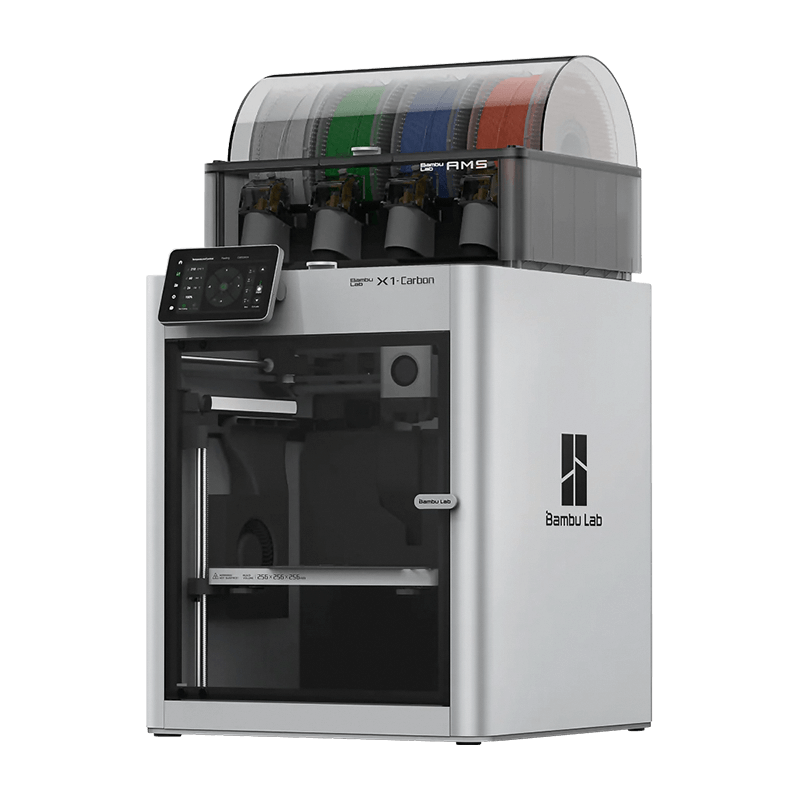
\includegraphics[width=0.8\linewidth]{images/3D-Drucker.png}
	\caption[Bambu Lab X1-Carbon 3 Pro]{Bambu Lab X1-Carbon 3 Pro}
	\label{fig:3D-Druck}
\end{figure}


\subsection{Vorteile des 3D-Drucks}
3D-Druck bietet viele Vorteile für Privatkunden und Unternehmen. Die nachfolgenden Vorteile zählen zu den wichtigsten:
\begin{itemize}
	\item Möglichkeit, komplexe Objekte relativ schnell herzustellen.
	\item Keine Vorlaufzeit nötig, d.h. keine Werkzeugproduktion erforderlich.
	\item Rapid Prototyping \emph{(deutsch „schnelle Prototypenherstellung“)}
	\item Kostengünstige Produktion
	\item Herstellung individueller Objekte
\end{itemize} \cite{3D-Druck-Vorteile}

\subsection{Nachteile des 3D-Druck}
3D-Druck bietet aber nicht nur Vorteile, sondern hat wie alle Technologien seine Nachteile und Schwächen.
\begin{itemize}
	\item Nachbearbeitung der Konstruktionen nötig.
	\item Nicht so genau wie subtraktive Fertigungverfahren.
	\item Lange Fertigungszeiten
	\item Begrenztes Bauvolumen
\end{itemize}
\cite{3D-Druck-Nachteile}

\subsection{Technische Voraussetzungen}
Um den 3D-Druck technisch durchführen zu können, werden folgende Komponenten benötigt:
\begin{itemize} 
	\item 3D-Drucker
	\item Slicer
	\item CAD-Programm
	\item 3D-Druck Material (Filament)
	\item Computer
\end{itemize}
Auf den nächsten Seiten wird auf diese Punkte näher eingegangen und ein Vergleich erstellt um die Vor- und Nachteile der genannten 3D-Drucker zu veranschaulichen. \cite{3ds}


\subsection{Druckverfahren}

Um Hardware mittels 3D-Drucks zu erstellen, gibt es verschiedene Möglichkeiten, das Ausgangsmaterial in die gewünschte Form zu bringen. Die gängigsten und weitverbreitesten Verfahren im Überblick: 

\begin{itemize}
	\item \textbf{FFF:} (Fused Filament Fabrication) oder \textbf{FDM} (Fused Deposition Modelling): Hierbei wird Kunststofffilament \emph{(eine einzelne Faser beliebig lang)} verwendet und Schicht für Schicht aufgetragen.
	\item \textbf{SLA:} Diese Technologie verwendet lichtempfindliches Kunstharz, das sich verfestigt. Wird ebenfalls Schicht für Schicht aufgetragen.
	\item \textbf{PBF:} Eine Möglichkeit, diese pulverbasierte Technologie zu nutzen, ist, das Pulver mittels Laser miteinander zu verschmelzen. 
\end{itemize}
\cite{kaffka} \cite{3ds}

\subsection{Werkstoffe}
3D-Drucker benötigen zum Drucken eines Objektes Material, das sie verbrauchen können, um das Objekt herzustellen. Im Rahmen dieser Diplomarbeit werden zwei Werkstoffe ganuer analysiert, nämlich Nylon und Kohlefaser.

\subsubsection{Nylon}
Nylon \emph{(techn. Polyamid)} ist ein langlebiges Material, das sich vorallem durch seine Widerstandfähigkeit gegen Hitze und mechanischen Außeneinwirkungen auszeichnet. Nylon gibt es in unterschiedlichen Ausführungen zb. als Filament, Draht oder Pulver mit unterschiedlichen Eigenschaften. \cite{Nylon}
\subsubsection{Kohlefaser}
Kohlefasern wird in Grundpolymeren wie PLA oder Nylon eingearbeitet um eine höhere Stabilität und Resistenz zu erzeugen wie zb. Nylon verstärkt mit Kohlefasern.\\
 \cite{Kohlefasern}


\subsection{3D-Drucker}

\subsubsection{Vergleich der 3D-Drucker}
Wie in der Einleitung des Kapitels \emph{"Hardware im Zusammenhang mit StageControl"} beschrieben, ist eine Möglichkeit zur Herstellung der benötigten Hardware das Drucken mittels eines 3D-Druckers. Um die bereits erwähnten 3D-Drucker (\emph{Bambu Lab X1-Carbon, Ultimaker 2 Extended+}) miteinander zu vergleichen, werden folgende Kriterien herangezogen: die Verarbeitbarkeit des Ausgangsmaterials und die Druckgeschwindigkeit bei einem Düsendurchmesser von 0,4 mm. 

Als Ausgangsmaterial wird bei beiden 3D-Druckern kohlefaserverstärktes Nylon-Filament verwendet.

\begin{table} [H]
	\begin{tabular}{ |p{2.7cm} |p{4.8cm}|p{4.8cm}| }
		\hline
		 \textbf{Kriterien} & \textbf{Ultimaker 2 Extended+}& \textbf{Bambu Lab X1-Carbon 3 Pro}\\
		\hline
		\textbf{Material} & Material kann verarbeitet werden & Material kann verarbeitet werden   \\ 
		\hline
		\textbf{Drucktempo} & Druckt mit einer Geschwindigkeit von 16mm\textsuperscript{3}/s &
		 Druckt mit einer Geschwindigkeit von 32mm\textsuperscript{3}/s   \\  
		\hline
		\textbf{Druckvolumen} & 223 x 223 x 205 mm & 256 x 256 x 256 mm \\
		\hline
		\textbf{Betriebssysteme} & MacOS, Windows, and Linux & Windows, MacOS \\
		\hline
	\end{tabular}
	\caption{Vergleich  Ultimaker 2 Extended+ und Bambu Lab X1-Carbon 3 Pro}
\end{table}
\cite{BambuLabX1-Carbon3DPrinter-Specifications}, \cite{Ultimaker2Extended+-Specification}

\subsection{Slicer}
\subsubsection{Was ist ein Slicer?}
Ein Slicer ist ein Stück Software, das es erst möglich macht 3D-Modelle auszudrucken, indem es einen sogenannten G-Code erstellt. G-Code ist die Programmiersprache, die von Computern verwendet wird, um mit Maschinen zu kommunizieren, wenn die Maschine Bewegungen ausführen soll. \\
\cite{Slicer_G-Code}


\section{CNC-Fräsen}

Ein weiterer Ansatz zur Hardware- bzw. Prototypenherstellung, der für StageControl benötigt wird, ist das CNC-Fräsen (\emph{engl. "Computerized Numerical Control"}). Diese Technologie wird vor allem in der metallverarbeitenden Industrie angewendet, da sie äußerst genau und kostengünstig arbeitet. Zudem beschränkt sich das CNC-Fräsen nicht nur auf Metall; es kann auch bei der Bearbeitung von Kunststoffen und Holz eingesetzt werden. Anders als bei der 3D-Druck-Technologie handelt es sich hier nicht um ein additives, sondern um ein subtraktives Verfahren.\\
 \cite{CNC-Fraesen} \cite{CNC-Fraesen_2} \cite{CNC-Fraesen_3}.


\begin{figure}[H]
	\centering
	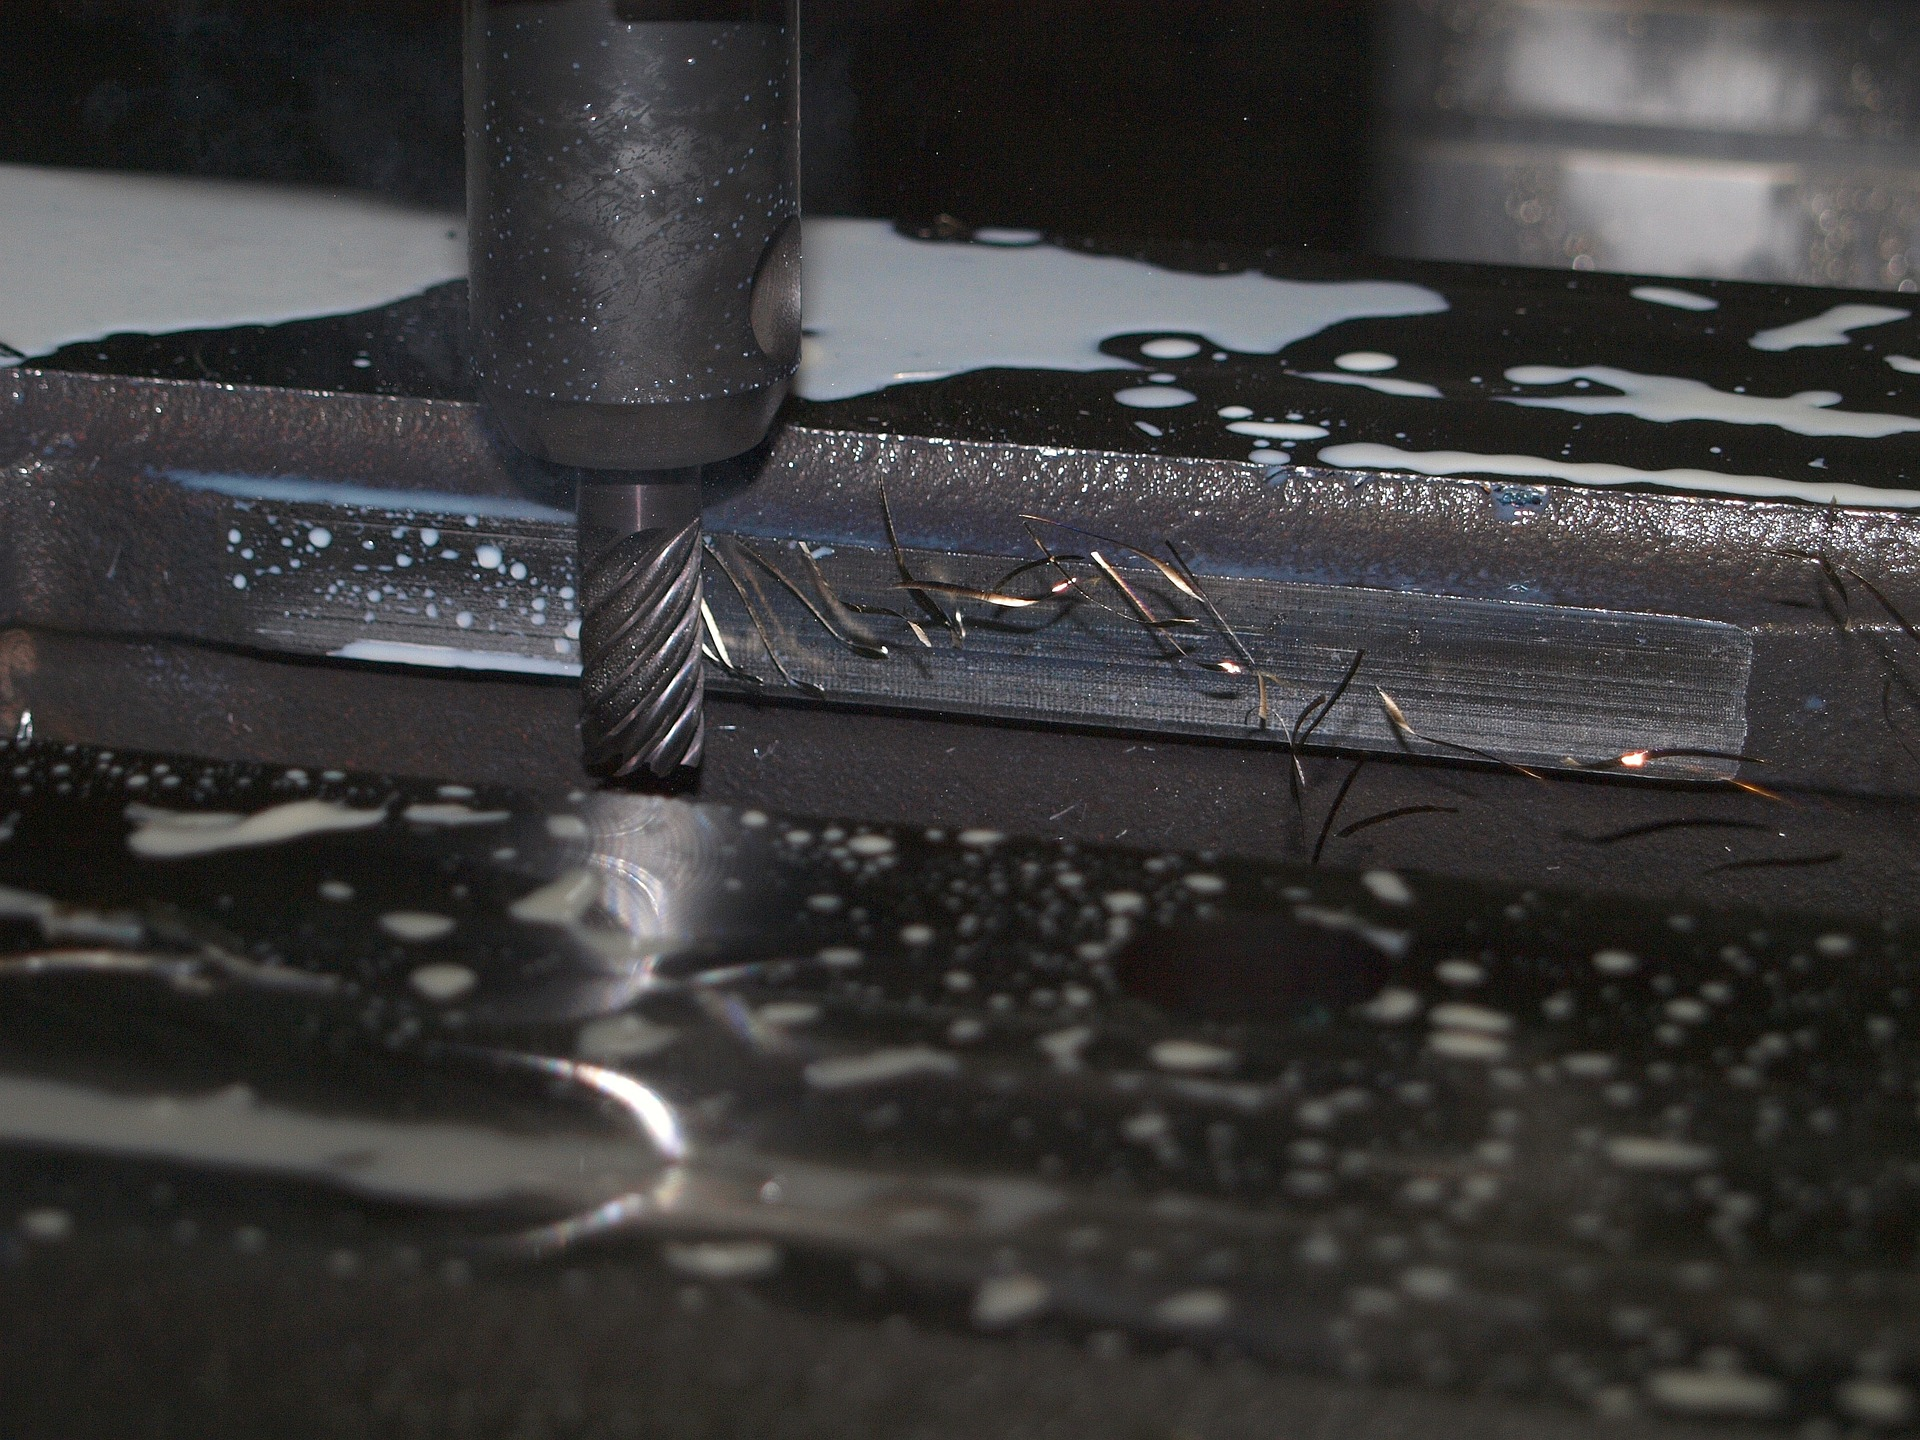
\includegraphics[width=0.8\linewidth]{images/CNC.jpg}
	\caption[CNC-Fräse]{CNC-Fräse}
	\label{fig:cnc-fraese}
\end{figure}

\subsection{Wie funktioniert CNC-Fräsen?}
Wie bereits in der Einleitung zum CNC-Fräsen erläutert, handelt es sich um ein subtraktives Verfahren, bei dem Material entfernt wird. Das Ausgangsmaterial wird fest in die Maschine eingespannt, während sich der Fräser bewegt. Der Fräser trägt dann das Material ab, um die gewünschte Form herzustellen. Um besonders präzise Abrundungen zu erzeugen, wird nicht das Material, sondern der Fräskopf fixiert, während sich das Material bewegt. Wie beim 3D-Druck wird hier auch G-Code als Steuerung der Maschine eingestzt. \\
\cite{CNC-Fraesen_2} \cite{CNC-Fraesen_3}.


\subsubsection{Einsatzmöglichkeiten}
CNC-Fräsmaschinen können vielseitig eingesetzt werden und eine Vielzahl von Objekten in unterschiedlichsten Größen und Formen herstellen. Zu den typischen Anwendungsbereichen zählen unter anderem:

\begin{itemize}
	\item Maschinenteilherstellung: Komponenten von Maschinen, die nur geringe Toleranzen zulassen.
	\item Prototypen: Herstellung von ersten Modellen in geringen Stückzahlen.
\end{itemize}

Durch den Einsatz von CNC-Fräsen können menschliche Fehler und die Ausschussrate minimiert werden. Dies führt zu niedrigeren Stückkosten, was sich besonders bei der Serienfertigung bemerkbar macht.\\
 \cite{CNC-Fraesen_2} \cite{CNC-Fraesen_3}.

\subsubsection{Vorteile des CNC-Fräsens}
CNC-Fräsen bietet im Vergleich zum herkömmlichen, manuellen Fräsen einige Vorteile. Wie bei jeder manuellen Arbeit können Arbeitsunfälle passieren. Durch den Einsatz moderner CNC-Fräsen, die aus der Ferne gesteuert werden können, lassen sich solche Unfälle reduzieren. Ein weiterer Vorteil des CNC-Fräsens ist seine gleichbleibende Genauigkeit, da die CNC-Fräse computergesteuert ist. Diese Technologie wird vor allem bei Werkstücken eingesetzt, die nur wenig Toleranz in der Genauigkeit zulassen. CNC-Fräsen arbeiten mit einer Präzision von 0,01 bis 0,03 mm. \\
\cite{CNC-Fraesen_Vorteile}

\subsection{CNC gesteuerte Maschinen}
Es gibt nicht nur CNC-Fräser oder Drehen, sondern alle Maschinen die durch CNC (\emph{engl. Computerized Numerical Control}) gesteuert werden, können als solche bezeichnet werden. Durch den Einsatz von CNC lassen sich die verschiedensten Maschinen computergestützt steuern. Zu diesen Maschinen zählen unter anderem CNC-Bohrmaschinen,  CNC-Laserschneidmaschinen, CNC-Schleifmaschinen, CNC-Wasserstrahlschneidmaschinen oder der 3D-Drucker. \\
\cite{Arten_CNC_Maschinen}

\subsection{Unterschied zwischen CNC-Fräsen und CNC-Drehen}
Beim CNC-Drehen wird ein Spannfutter anstatt des Schneidewerkzeugs eingesetzt. Dies ermöglicht die Herstellung von runden, zylindrischen oder konischen Formen. Mit diesem Verfahren lassen sich keine Objekte herstellen die eine hohe Präzision erfordern. Im Gegensatz zur CNC-Fräsmaschine arbeitet das CNC-Drehen nur auf zwei Achsen. Zudem dreht sich das Material und der Fräser ist fixiert, so wird das Material wie bei der CNC-Fräse abgetragen. \\
\cite{CNC-Drehen_Unterschied}


\subsection{Werkstoffe}
Bei der CNC-Fräsung können die unterschiedlichsten Materialien verwendet werden. Materialien, die eine CNC-Fräse verarbeiten kann, sind zerspanbar. Zu den gängigsten zählen:

\begin{itemize}
	\item Metalle, z. B. Stahl, Aluminium, Titan, Bronze, Messing.
	\item Holz => Drechseln
	\item Zerspanbare Kunststoffe, z. B. PEI (\emph{Polyetherimid}), die sich durch ihre mechanische Festigkeit und Steifigkeit auszeichnen.
\end{itemize}
\cite{CNC-Fraesen_3} \cite{PEIZerspannung} \cite{PEIKunststoff-Polyetherimid}

\subsection{Fertigungsmöglichkeiten}

\subsubsection{3-Achs-Fräsung}
Hierbei kann sich der Fräser auf drei Achsen bewegen, nämlich auf der X-, Y- und Z-Achse. So kann das Material von allen drei Seiten bearbeitet werden. Es handelt sich um das einfachste Fräsverfahren. Zwar können auch komplexere Objekte erstellt werden, dies erfordert jedoch ein mehrfaches Umspannen des Werkstücks.

\subsubsection{4-Achs-Fräsung}
Zusätzlich zu den bereits bekannten drei Achsen kann nun eine vierte Achse integriert werden, nämlich das Schwenken der Aufspannung des Frästeils. Dadurch kann das Umspannen, das bei der 3-Achs-Fräsung notwendig ist, vermieden werden.

\subsubsection{5-Achs-Fräsung}
Bei der 5-Achs-Fräsung kann nicht nur die Aufspannung des Frästeils zum Schwenken gebracht werden sondern auch der Maschinentisch selbst ist rotierbar. So kann das Werkstück von 5 Seiten in einer Aufspannung bearbeitet werden. Diese Fräsen werden bei der Produktion höchstkomplexer Strukturen eingestzt.\\
\cite{Fraesen-3/4/5-Achs}


\section{3D-Modellierungsprogramme}
Auf dem Markt rund um 3D-Modellierungsprogramme gibt es eine große Auswahl an den verschiedensten Programmen. Vom anfängerfreundlichen Tinkercad, das durch seine einfache Bedienbarkeit und zahlreiche Tutorials überzeugt, bis hin zu einem der führenden CAD-Programme wie Catia, das in der Industrie für seine leistungsstarken und umfangreichen Funktionen geschätzt wird, ist alles dabei. Im Rahmen dieser Diplomarbeit wurden einige der Marktführer recherchiert und miteinander verglichen. \\
\cite{CAD-Programme}, \cite{3D-Printing-Software}

\subsection{Vergleich verschiedener Software}

\subsubsection{Autodesk Fusion}
Es eröffnet zahlreiche Anwendungsmöglichkeiten, die von der Prototypenerstellung bis hin zur Entwicklung von Konsumgütern reichen. Dieses Programm bietet umfangreiche Werkzeuge für Design, Engineering und Fertigung.  Fusion 360 wird von vielen internationalen und nationalen Unternehmen verwendet, weil es vielseitig einsetzbar ist und sowohl in kleinen als auch in großen Projekten hervorragende Unterstützung bietet. Dank seiner cloudbasierten Plattform ermöglicht Fusion 360 eine nahtlose Zusammenarbeit und den einfachen Austausch von Projektdaten, was es zu einer bevorzugten Wahl in der modernen Produktentwicklung macht. \\
\cite{AutodeskFusion}

\textbf{Vorteile}
\begin{itemize}
	\item Genutzt von vielen namhaften Unternehmen wie zb. Yamaha oder Panasonic
	\item Große Community
	\item Kostenlose Version für Schulen
\end{itemize} 

\textbf{Nachteile}
\begin{itemize}
	\item Cloud Based; Kann zu Problemen führen, wenn offline genutzt 
	\item Benötigt eine schnelle Internetverbindung
	\item Hoher Anspruch an die Hardware des Computers
\end{itemize}
\cite{AutodeskFusionReviews}


\subsubsection{Blender} 
Blender bietet vielseitige Anwendungsmöglichkeiten, von Modellierung und Animation bis hin zur Spieleentwicklung und visuellen Effekten. Dieses Open-Source-Programm bietet umfassende Werkzeuge für Modellierung, Simulation, Rendering, Compositing und Motion Tracking. Zudem wird Blender von vielen internationalen und nationalen Unternehmen sowie unabhängigen Kunden bzw. Kundinnen verwendet, weil es viele Einsatzmöglichkeiten bietet und gratis zugänglich ist. Dank seiner aktiven Community und regelmäßigen Updates bleibt Blender immer auf dem neuesten Stand der Technik. \\
\cite{Blender}

\textbf{Vorteile}
\begin{itemize}
	\item Gratis 
	\item Open Source Software
	\item Funktioniert auf allen gängigen Betriebssystemen
	\item Regelmäßige Updates
	\item große Community
\end{itemize}

\textbf{Nachteile}
\begin{itemize}
	\item Kein Industriestandard - wird nicht von großen Unternehmen genutzt
	\item Nicht die benutzerfreundlichste Oberfläche
\end{itemize}
\cite{BlenderPros&Cons}


\subsubsection{FreeCAD}
FreeCAD hat vielseitige Anwendungsmöglichkeiten, von der Modellierung bis hin zur Erstellung technischer Zeichnungen und Simulationen. Diese Open-Source-Software bietet umfassende Werkzeuge für Ingenieure, Architekten, Produktdesigner und Privatkunden. Zudem wird FreeCAD von vielen Unternehmen sowie unabhängigen Entwicklern und Entwicklerinnen genutzt, weil es flexible Einsatzmöglichkeiten bietet. Durch seine modulare Architektur und der aktiven Community wird FreeCAD kontinuierlich weiterentwickelt und verbessert. \\
\cite{FreeCAD}  \cite{FreeCAD_2}

\textbf{Vorteile}
\begin{itemize}
	\item Open Source Software
	\item Gratis
	\item Funktionsfähig für alle gängigen Betriebssysteme
	\item Aktive Community	 
\end{itemize}

\textbf{Nachteile}
\begin{itemize}
	\item weniger Nutzer und Nutzerinnen als die bereits genannten Programme
	\item kein Industriestandard
	\item limitierte Funktionalitäten im Vergleich zu Bezahlsoftware
\end{itemize}
\cite{FreeCADReviews}

\subsubsection{Autodesk Tinkercad}
Autodesk Tinkercad ist ein für Anfänger und Anfängerinnen und Schüler und Schülerinnen entwickeltes Online-Tool. Wie der Name es schon verrät, ist es ein Produkt von Autodesk, wie das vorher genannte Autodesk Fusion 360. Dieses webbasierte Programm erfüllt alle grundlegenden Anforderungen und bietet intuitive Werkzeuge für Schüler und Schülerinnen, Lehrer und Lehrerinnen und Privatpersonen. Zudem wird Tinkercad von vielen Bildungseinrichtungen verwendet, weil es leicht zugänglich und einfach zu erlernen ist. Dank seiner klaren Benutzeroberfläche und umfangreichen Tutorials ermöglicht Tinkercad einen schnellen Einstieg in die Welt des 3D-Designs und der Elektronik. \\
\cite{Tinkercad}

\textbf{Vorteile}
\begin{itemize}
	\item Gratis
	\item Benutzerfreundliches UserInterface (\emph{Nutzeroberfläche})
	\item intuitives Design
	\item Online Tool - kein Download 	
	\item viele einsteigerfreundliche Tutorials 
\end{itemize}

\textbf{Nachteile}
\begin{itemize}
	\item Weniger professionell
	\item kein Industriestandard 
\end{itemize}
\cite{TinkercadReviews}

\section{Mischpult}
 Für StageControl benötigen wir zur Ansteuerung einer Tonanlage ein Mischpult, um den von uns gewünschten Stereoeffekt zu erzeugen. Mischpulte, auch Mixer genannt, gibt es in ganz unterschiedlichen Größen. Die Größe hängt meist von der Anzahl der Kanäle ab, die das Mischpult bietet. Mischpulte werden immer dann verwendet, wenn mehrere Audiosignale verarbeitet werden müssen, wie auf Bühnen oder in Proberäumen. Bei allen Mischpulten gibt es eine sogenannte Leserichtung, die den Aufbau des Mischpults beschreibt. Von links nach rechts findet man die einzelnen Kanäle, und von oben nach unten die Bearbeitungsmöglichkeiten des Tons. Dazu kommt noch der sogannte Masterbereich. Hier wird alles gesteuert, was zentral gereglt werden muss. Diese Einstellungen gelten dann für alle Kanäle. \\
\cite{Mischpult_Information}  \cite{Mischpult_Master}

\begin{figure}[H]
	\centering
	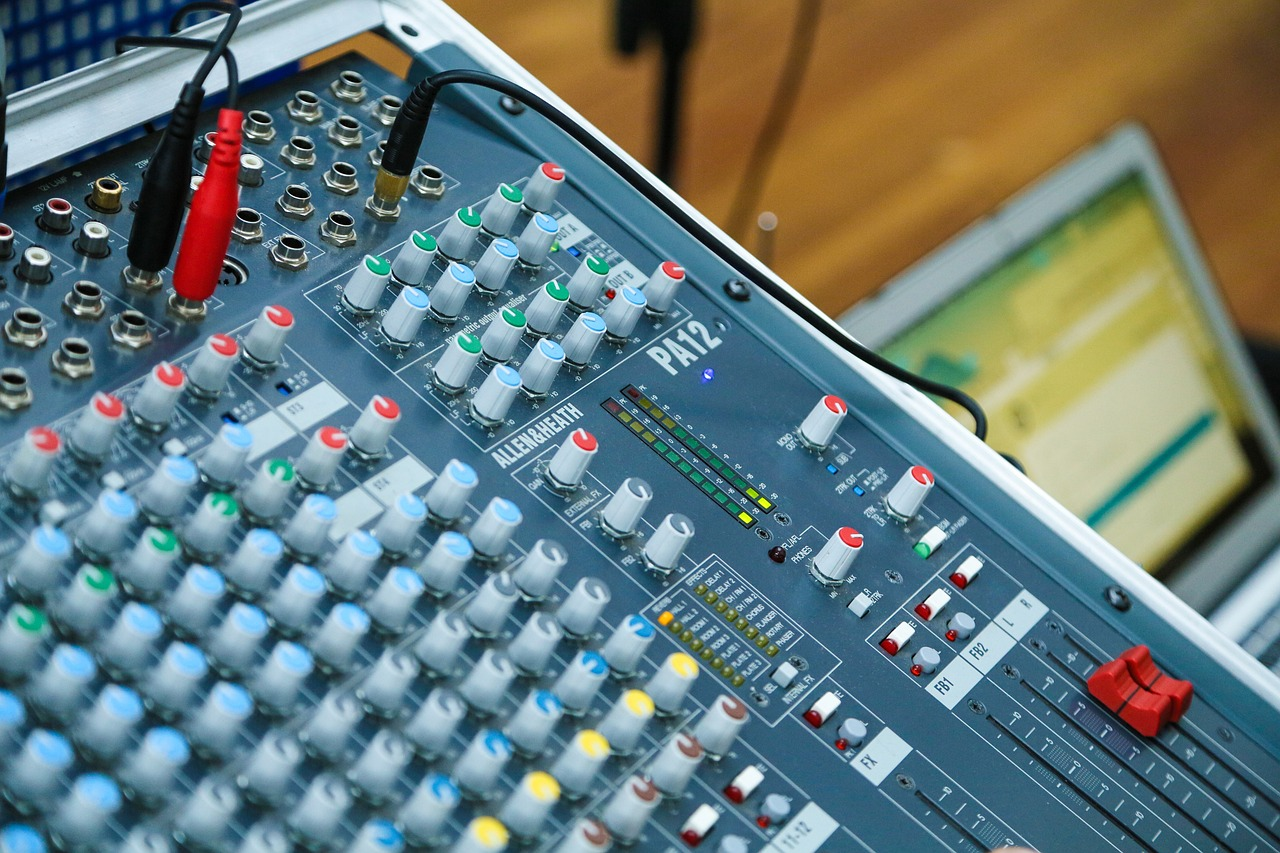
\includegraphics[width=0.8\linewidth]{images/mischpult.jpg}
	\caption[Mischpult]{Mischpult}
	\label{fig:Mischpult}
\end{figure}

\subsection{Funktionsweise eines Mischpults}
Im Grunde summiert ein Mischpult alle Tonquellen zu einen einzigen Signal. So kann dann dieses Signal über die Tonanlage ausgegeben werden. Bei Mischpulten gibt es eine Vielzahl von Knöpfen und Reglern für jeden Kanal, diese sind wie schon erwähnt zur Bearbeitung des Tones da, im Rahmen dieser Diplomarbeit wird auf dies nicht genauer eingagangen. \\
\cite{Mischpult_Erklaerung}

\subsection{Einsatzmöglichkeiten}
Mischpulte finden eine Vielzahl von Anwendungsmöglichkeiten, wie z.B. auf Bühnen oder in Proberäumen. Mischpulte übernehmen eine Bandbreite von Aufgaben. Die folgenden gehören zu den Wichtigsten:
\begin{itemize}
	\item Signalverstärkung
	\item Bearbeitung von Signalen
	\item Signale zum Aufnahmesystem schicken
\end{itemize}
\cite{Mischpult_Verwendungszweck}

\subsection{Unterschied Digital/Analog}
\subsubsection{Digital}
Unter einem digitalen Mischpult versteht man ein Mischpult, das analoge Signale in digitale Signale umwandelt und diese Signale mittels Software bearbeitet. Um ein digitales Signal wieder über eine Tonanlage auszugeben, muss es erneut in ein analoges Signal umgewandelt werden. Dies führt wiederum zu Latenzzeiten bei der Signalausgabe.
\subsubsection{Analog}
Im Gegensatz dazu steht das analoge Mischpult. Es wandelt die Signale nicht in digitale um, sondern behält deren ursprüngliche analoge Form bei und bearbeitet sie ohne Software weiter. Ohne diese Umwandlung gibt es nahezu keine Latenzzeit bei der Ausgabe der Signale. \\
\cite{Mischpult_Analog/Digital}

\subsection{Anforderungen für StageControl}
Für StageControl ist es besonders wichtig, dass das verwendete Mischpult entweder jeden Kanal einzeln panen (\emph{Regler zu Ausrichtung des Tons (links/Rechts)}) kann oder das der Master mindestens zwei Lautsprecher einer Tonanlage einzeln ansteuern kann. Somit kann der von uns gewünschte Stereoeffekt erzeugt werden.

\subsection{Vergleich zweier Modelle}
Wie am Anfang des Kapitels \emph{Mischpult} beschrieben benötigt StageControl ein Mischpult, um den von uns gewünschten Stereoeffekt zu erzeugen. Hierzu werden zwei Mischpulte herangezogen, die unseren Kriterien entsprechen und  verglichen.

\begin{table} [H]
	\begin{tabular}{ |p{3.1cm} |p{4.8cm}|p{4.8cm}| }
		\hline
		\textbf{Kriterien} & \textbf{Behringer Xenyx 1204USB}& \textbf{the t.mix xmix 1402 USB}\\
		\hline
		\textbf{Kosten} & 169€ & 168€  \\ 
		\hline
		\textbf{Digital/Analog} & Analog & Analog   \\  
		\hline
		\textbf{Master kann zwei Lautsprecher seperat ansprechen} & Ja & Ja \\
		\hline
		\textbf{PC-Schnittstelle} & USB-B & USB-B  \\
		\hline
		\textbf{Gewicht}& 2.8 kg & 4.8 kg \\
		\hline	
	\end{tabular}
	\caption{Vergleich Behringer Xenyx 1204USB und the t.mix xmix 1402 USB} 
\end{table} 
\cite{Mischpult_Kriterien_1204}, \cite{Mischpult_Kriterien_1402}

\section{Lichtsteuerung}
Ein weiterer Aspekt dieser Diplomarbeit ist die gleichzeitige Ansteuerung von Ton- und Lichtanlagen, wie z.B. einem Spotlight (\emph{deutsch Verfolgungsscheinwerfer}), das den Künstler bzw. der Künstlerin auf der Bühne verfolgt. Auf Bühnen wird nicht nur ein Spotlight eingesetzt, sondern ganze Anlagen von Lichtern. Dies wird gemacht, um für den Zuschauer eine immersive Vorstellung zu bieten. 

\begin{figure}[H]
	\centering
	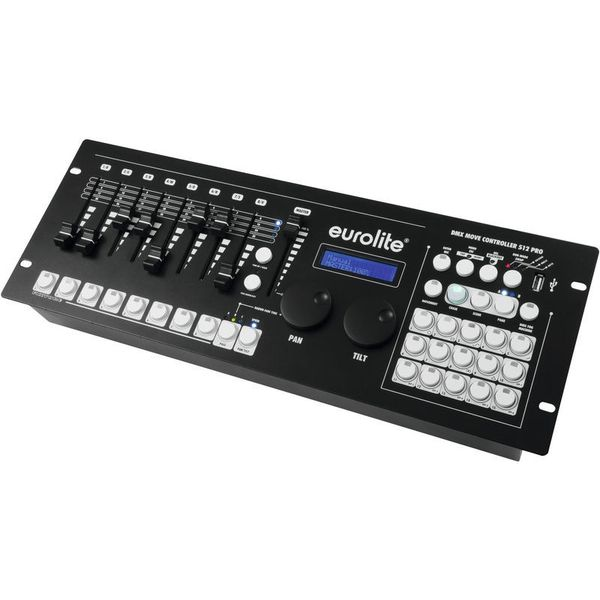
\includegraphics[width=0.7\linewidth]{images/DMX_Controller.jpg}
	\caption[DMX Controller]{DMX Controller}
	\label{fig:DMX_Controller}
\end{figure}

\subsection{Lichtanlagen bei StageControl}
Im Fall von StageControl wird keine vollständige Lichtanlage verwendet; es kommt lediglich ein Scheinwerfer zum Einsatz, um die Beleuchtung des Künstlers bzw. der Künstlerin via Positionsverfolgung zu ermöglichen. So erhalten wir die genaue Abstimmung von Ton und Licht auf die Person.

\subsection{Ansteuerung von Lichtanlagen}
Die gängigsten Arten der Ansteuerung von Lichtanlagen sind das DMX-Protokoll (\emph{Digital Multiplex}) oder das RDM-Protokoll (\emph{Remote Device Management}). Zur Ansteuerung der Lichtanlagen selbst wird ein DMX-Controller benötigt, der die Scheinwerfer steuert. Es wird ein DMX-Controller mit einem DMX-Ausgang und ein Scheinwerfer mit einem DMX-Eingang gebraucht.\\
\textbf{DMX} ist das am häufigsten verwendete Protokoll zur Lichtansteuerung in der Bühnentechnik. Moving-Heads, Lichteffekte und viele mehr werden in der Regel mithilfe von Lichtsteuerpulten über das DMX-Protokoll angesteuert und/oder programmiert.\\
\textbf{RDM} basiert auf dem DMX-Protokoll, erlaubt aber im Halbduplexbetrieb Rückmeldungen, was das Einrichten deutlich erleichtern kann.\\
\cite{Lichtanlage_RDM_DMX}

\subsection{Hartes bzw. weiches Licht}
Es gibt zwei Lichtarten, die man in der Lichttechnik unterscheiden kann, nämlich hartes und weiches Licht. Beide Arten bieten sich für unterschiedliche Einsatzmöglichkeiten an. Weiches Licht wird meist eingesetzt, um größere Bereiche auszuleuchten. Auf der anderen Seite der Lichtskala gibt es das harte Licht, das sehr präzise eingesetzt werden kann, wie im Fall von StageControl bei der Verfolgung des Künstlers/der Künstlerin auf einer Bühne. Bei Scheinwerfern, die hartes Licht ausstrahlen, kommt das Licht von einem Punkt aus. Hingegen wird weiches Licht von einer Fläche aus abgestrahlt.\\
\cite{Hartes_Weiches_Licht}

\subsection{Arten von Scheinwerfern}
In der Lichttechnik gibt es verschiedenste Scheinwerfertypen, die unterschiedliche Aufgaben besonders gut erfüllen. Zwei Scheinwerfertypen, die im Rahmen dieser Diplomarbeit zum Einsatz kommen, werden genauer erklärt.

\subsubsection{Verfolgerscheinwerfer}
Der Verfolgerscheinwerfer wird verwendet, um Personen auf Bühnen zu verfolgen. Diese Scheinwerfer werden nicht wie andere Scheinwerfer fix montiert, sondern lassen sich bewegen, um den gewünschten Verfolgungseffekt zu bieten. Dies geschieht nicht automatisch, sondern wird manuell von einem Beleuchter während der Show durchgeführt. Es gibt verschiedene Lösungsansätze zur Bewegung von Movinglights (\emph{deutsch „Bewegbare Lichter“}). \ Bei Konzerten wird ein Verfolgerscheinwerfer oberhalb der Bühne gemeinsam mit dem Beleuchter platziert. Dieser steuert dann das Licht über ein Bedienfeld während der Performance.\\
\cite{Verfolgerscheinwerfer}

\begin{figure}[H]
	\centering
	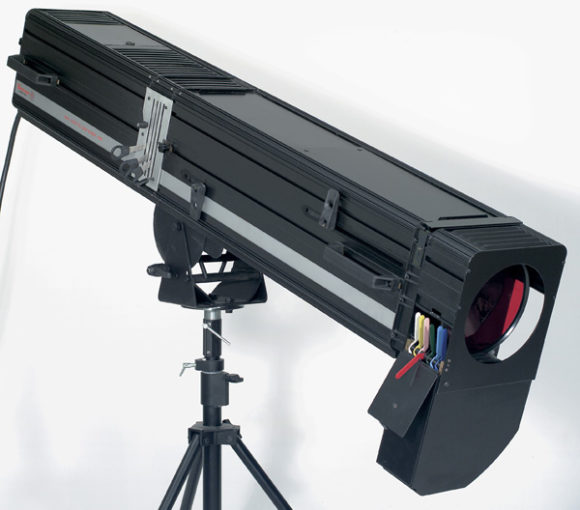
\includegraphics[width=0.7\linewidth]{images/Verfolgerscheinwerfer.jpg}
	\caption[Verfolgerscheinwerfer]{Verfolgerscheinwerfer}
	\label{fig:Verfolgerscheinwerfer}
\end{figure}

\subsubsection{Profilscheinwerfer}
Dieser Scheinwerfertyp wird vor allem im Theaterbereich eingesetzt. Ein enormer Vorteil des Profilscheinwerfers ist, dass er ein hartes und exaktes Licht ausstrahlt. Außerdem ist das Streulichtaufkommen deutlich geringer als bei anderen Scheinwerfern. Streulicht ist das Licht, das außerhalb des eigenlichen Lichtkegels auftritt. Zudem verfügen Profilscheinwerfer über einen Zoom, der manuell oder automatisch erfolgen kann. Dieser Scheinwerfertyp bietet zusätlich eine Scharfstellfunktion/Fokus mittels Linsenverschiebung an, diese wird durch den Linsentubus ermöglicht.\\
\cite{Profilscheinwerfer}

\begin{figure}[H]
	\centering
	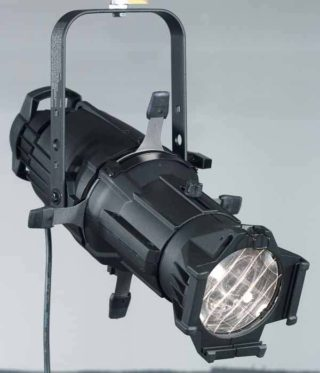
\includegraphics[width=0.7\linewidth]{images/Profilscheinwerfer.jpg}
	\caption[Profilscheinwerfer]{Profilscheinwerfer}
	\label{fig:Profilscheinwerfer}
\end{figure}

\section{Servomotoren}
\subsection{Einsatz von Servos bei StageCotrol}
Servomotoren werden für die Umwandlung der physischen Bewegung des Künstlers, in mechanische Bewegung des Servomotors benötigt, um so die Regler des Mischpults in Abstimmung und Ausrichtung des Künstlers mit dem Ton zu automatisieren. Diese Servomotoren werden oberhalb des Mischpult mithilfe des Gerüsts plaziert, wie in Kapitel 2.2.1 beschrieben. Diese Motoren sind essenziell für den Erfolg, da ohne diese Servos keine Automatisierung erfolgen kann.

\subsection{Was ist ein Servomotor}
Unter einem Servomotor wird keine Bauart eines Motors verstanden, sondern vielmehr spezielle Eigenschaften. Diese Eigenschaften sind: Strom-, Drehzahl- und/oder Positionsgeregelt. Ein Servomotor ist immer elektrisch betrieben. Diese Motoren geben Rückmeldungen an die Regelelektronik. Diese Rückmeldungen enthalten Informationen über Winkelposition der Motorwelle, der Drehgeschwindigkeit und der Beschleunigung. Die Regelelektronik kann anhand dieser zurückgemeldeten Daten wieder die Daten der Sollparameter an den Motor schicken, die zuvor eingegeben wurden. \\
\cite{Servomotor_Info}

\subsection{Anforderungen für StageControl}
Für den Einsatz bei StageControl gibt es Vorraussetzungen, die die Servomotoren erfüllen müssen, ehe sie in Erwägung gezogen werden. Diese Kriterien sind: Drehung des Motors im und gegen den Uhrzeigersinn, Kompaktheit, passenende Schnittstelle (Bus/Analog/Digital) für die Eingabe der Sollzustände und die Rückmeldung der Aktuellen Position.

\begin{figure}[H]
	\centering
	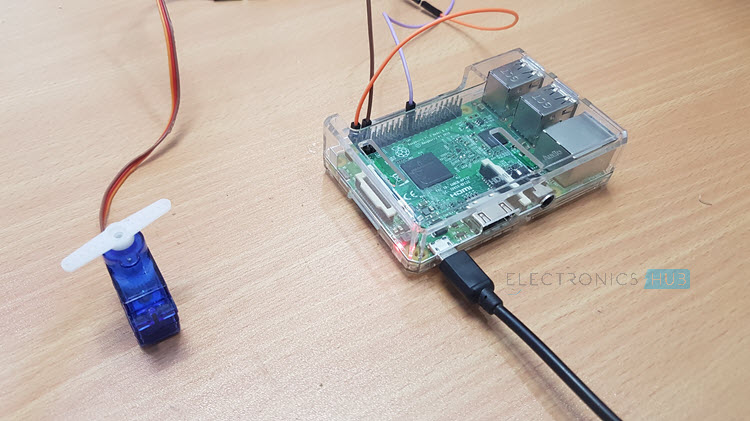
\includegraphics[width=0.7\linewidth]{images/servo.jpg}
	\caption[Servomotor]{Servomotor}
	\label{fig:Servo}
\end{figure}

\subsection{Arten von Servomotoren}
Es gibt einige unterschiedliche Arten von Servos, die wichtigsten drei sind: Gleichstrom, kernlose und bürstenlose Motoren. \\
Bei Gleichstromservos handelt sich um die billigste und gängiste Art der Motoren. Dieser Servotyp besteht aus Eisenkernen um die Kupferdraht gewickelt ist, sowie einem Kommutator Ring und Bürsten. Diese Bürsten werden zur Umschaltung der Felder benötigt und einem Gehäuse. \\
Kernlose Motoren sind erheblich teuerer in der Produktion als Gleichstrommotoren, da diese aus teurern Materialien bestehen. Ihr großer Vorteil gegenüber herkörmlicher Gleichstrommotoren ist, das diese deutlich schneller beschleunigen und abbremsen können. \\
Anstelle der Bürsten und dem Metallring bei Bürstenservos, wird bei den Bürstenlosen Servos Elektronik, die den Motor steuert, eingebaut um die selbe Zuverlässigkeit zu gewährleisten. Der Einbau von Elektronik zeichnet sich durch die längere Lebensdauer des Servos aus. Durch die Elektronik fallen diese Motoren deutlich teurer aus als Gleichstrommotoren. \\
\cite{Servomotor_Arten}


\subsection{Ansteuerung von Servos}
Servomotoren werden über ein sogenanntes PWM-Signal (\emph{Pulsweitenmodulations-Signal}) gesteuert. Dies bedeutet, dass der Servomotor über elektrische Pulse angesteuert wird und so die Befehle erhält, auf welche Postion er fahren muss. Diese Motoren werden üblicherweise über drei Kabeln mit dem Steuerunggerät verbunden. Das erste Kabel ist das Massekabel, dies ist für die Rückleitung der Pulse verantwortlich. Nummer zwei ist das Versorgungsspannungskabel, dies versorgt den Servomotor mit der nötigen elektrischen Spannung. Das dritte Kabel ist das Signalleitungskabel, dieses Kabel leitet die Pulse an den Servo weiter, so wird dem Servo die anzufahrende Position mitgeteilt.\\
\cite{Servomotor_Ansteuerung}

\section{Navigation}

Um die Licht- und Audioanlagentechnik richtig zu koordinieren benötigt man eine Art von Navigation. Da es sich meist um Bühnen im Innenbereich handelt, kann man keine übliche Technologie verwenden.


\subsection{GPS}
GPS (\emph{=engl. Global Positioning System}) wird für die Standortermittlung im Außenbereich verwendet und ist für unseren Fall nicht verwendbar. Für die genaue Bestimmung von Positionen werden Satelliten verwendet.
\cite{GPS}

\textbf{Funktionsweise des GPS}

Es gibt GPS-Satelliten die, die Erde zweimal pro Tag umkreisen in einer genauen Umlaufbahn. Diese Satelliten senden eindeutige Signale und Bahnparameter aus, somit können die genauen Postionen der GPS-Geräte bestimmt werden. 
In so gut wie jeden neuen Geräten ist das GPS-standart und werden für die verschiedensten Funktionen verwendet. Durch die Positionsermittlung können folgende andere Informationen berechnet werden:

\begin{itemize}
	\item Geschwindigkeit
	\item Peilung
	\item Track
	\item Reisedistanz
	\item Distanz zum Ziel
	\item Zeiten von Sonnenaufgang und Sonnenuntergang
\end{itemize}

\textbf{Signal}

Wenn GPS-Signale die Erde erreichen, sind die gesendeten Signale sehr schwach. Deshalb kommt es auch zu Problemen beim Durchdringen von Objekten wie Gebäuden o. Ä. Bei modernen GPS-Empfängern ist eine Indoor-Ortung möglich.

\textbf{Fehlerquellen für die Genauigkeit der GPS-Signale}

Es gibt einige relevante Fehlerquellen für GPS-Signale darunter fallen:
\begin{itemize}
	\item Position der Satelliten
	\item Signaleffekt der Umgebung
\end{itemize}

\textbf{Position der Satelliten}

Um ein Objekt zu positionieren sind mindestens drei Satelliten notwendig und einen weiteren, um etwägige Fehler zu beseitigen. Grundsätzlich gilt: Desto mehr Satelliten, desto genauer die GPS-Genauigkeit. Außerdem sollte das Signal von gleichmäßig verteilten Satelliten kommen, ist die GPS-Genauigkeit höher. Für die Berechnung dieser Genauigkeit gibt es den Dilution of Precision (= DOP) Wert.  Je kleiner dieser Wert, desto genauer ist das GPS-Signal.
\begin{figure}[H]
	\centering
	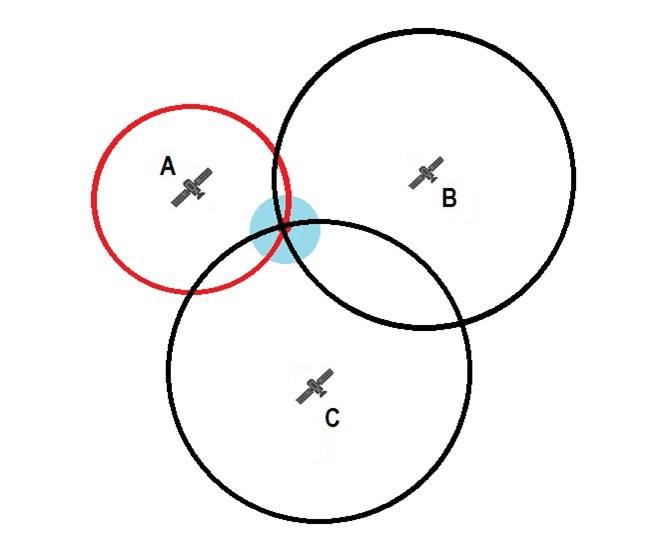
\includegraphics[width=0.7\linewidth]{images/Satellitenposition.jpg}
	\caption[Satellitenpositionierung]{Satellitenpositionierung}
	\label{fig:Satellitenposition}
\end{figure}

\textbf{Signaleffekt der Umgebung}

Bis die Signale von Satelliten schlussendlich beim GPS-Empfänger ankommen legen sie eine lange Stecke zurück, die Ausbreitungsumgebung beinflusst nicht nur die Siganlestärke, sondern auch die Genauigkeit, stark. 
\begin{figure}[H]
	\centering
	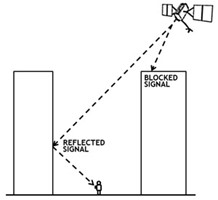
\includegraphics[width=0.7\linewidth]{images/Satelliteneinfluss.jpg}
	\caption[Satelliteneinfluss]{Satelliteneinfluss}
	\label{fig:Satelliteneinfluss}
\end{figure}
\cite{GPS Fehlerquellen}

\subsection{ESP32}

ESP32 ist eine Reihe von Chip-Mikrocontrollern, die von dem Unternehmen Espressif entwickelt wurden und mit Hilfe von Arduino kommunizieren. Der ESP32 zeichnet sich mit folgenden Dingen aus:

\begin{itemize}
	\item niedrige Anschaffungskosten
	\item geringer Stromverbrauch
	\item Wi-Fi
	\item Bluetooth
\end{itemize}


\begin{figure}[H]
	\centering
	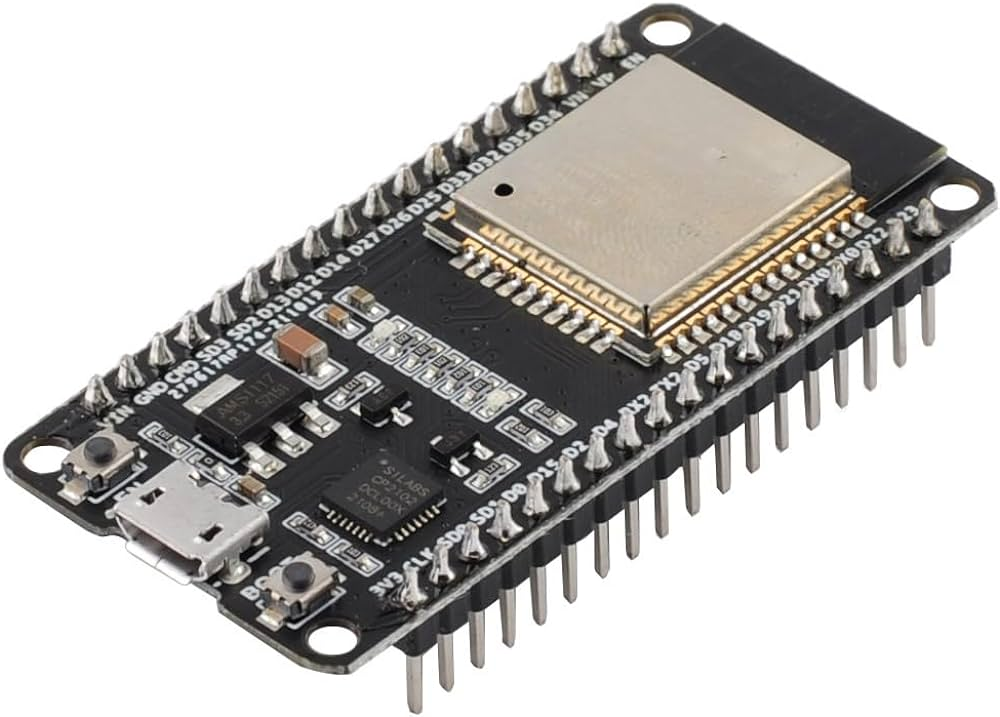
\includegraphics[width=0.7\linewidth]{images/ESP32.jpg}
	\caption[ESP32]{ESP32}
	\label{fig:ESP32}
\end{figure}

\textbf{Anschaffungskosten \& Stromverbrauch}

Der Mikrocontroller ist bereits ab einem Preis von \$6 erhältlich. Außerdem verbraucht dieser im Vergleich zu anderen Mikrocontrollern sehr wenig Strom und unterstützt Energiesparmodule, wie Tiefschlaf.

\textbf{Funktionen}

Der Mikrocontroller bietet nicht nur Wi-Fi (\emph{=Wireless Local Area Network}), sondern auch Bluetooth. Mit der Wireless Local Area Network Funktionen kann man einfach und drahtlos eine Verbindung zu einem Netzwerk herstellen und somit eine Kommunikation von vielen Geräten möglich machen. Außerdem verfügt der Mikrocontroller über Bluetooth-Classic.

\subsection{ESP32-Spezifikationen}

\begin{itemize}
	\item Bluetooth Classic und Bluetooth Low Energy
	\item Tensilica Xtensa Dual-Core 32-Bit LX6 Mikroprozessor, 160 oder 240 MHz
	\item ROM:  448 KB
	\item SRAM:  520 KB 
\end{itemize}
\cite{ESP32}

\subsection{MPU-6050}

Für weitere Funktionen benötigt man z.B. die Erweiterungsplatine MPU-6050, diese bringt einen Beschleunigungssensor und ein Gyroskop mit. Diese Platine beläuft sich auf einen Preis von ca. \$3.

\begin{figure}[H]
	\centering
	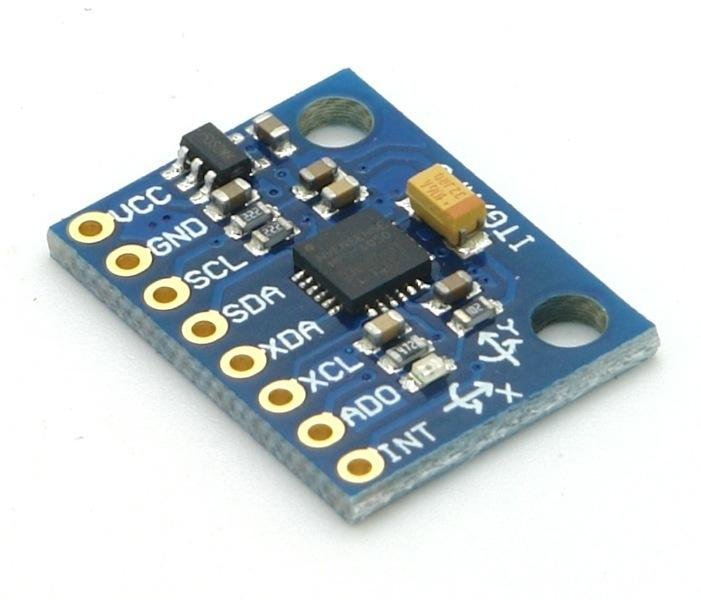
\includegraphics[width=0.7\linewidth]{images/MPU6050.jpg}
	\caption[MPU6050]{MPU-6050}
	\label{fig:MPU6050}
\end{figure}


\textbf{Gyroskop}

Jeder kennt die Wirkung eines Kreisel, ein Gyroskop hat genau diese und wird deshalb auch Kreiselinstrument genannt. Man nutzt die Wirkung, um die Lage eines Objektes zu bestimmen. Im Falle von einem MPU-6050 wird ein Sensor namens Micro-Electric-Mechanical Systems (\emph{kurz MEMS}) verwendet. 


\begin{figure}[H]
	\centering
	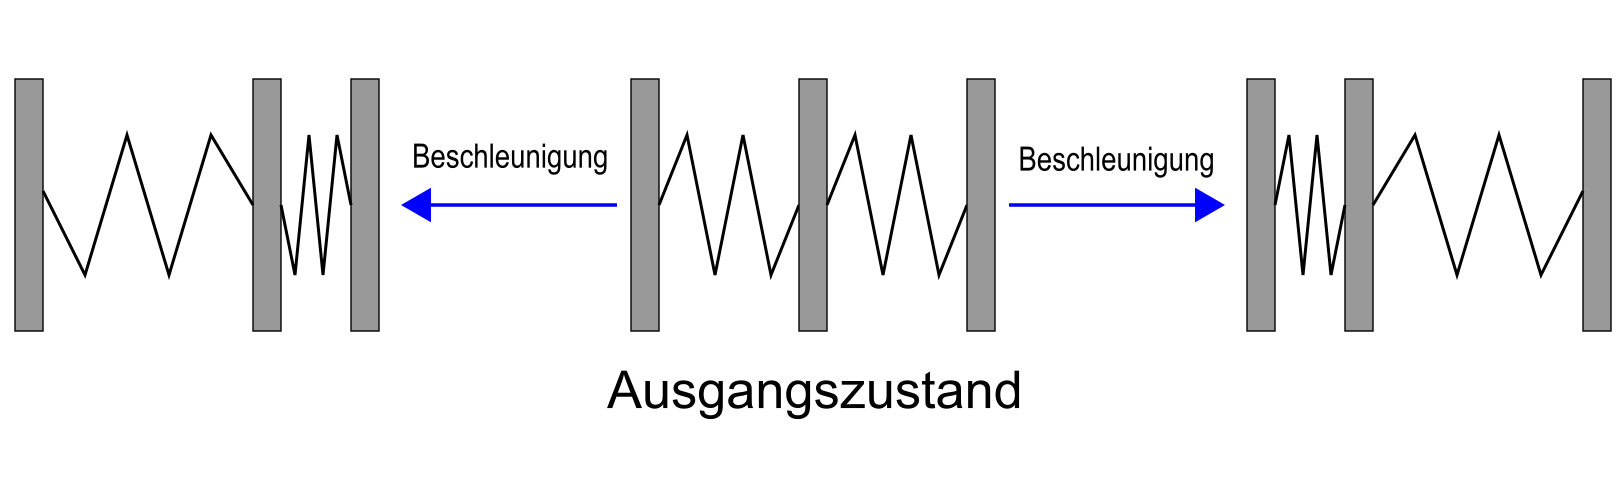
\includegraphics[width=0.7\linewidth]{images/Beschleunigungssensor.png}
	\caption[Beschleunigungssensor]{Beschleunigungssensor}
	\label{fig:Beschleunigungssensor}
\end{figure}

\textbf{Beschleunigungssensor}

Ein Beschleunigungssensor funktioniert nach dem selben Prinzip, wie ein Gyroskop. Der einzige Unterschied ist, dass der Sensor die Beschleunigung in Richtung der x-, y- und z-Achse deklariert. Ein Gyroskop bezieht sich lediglich auf die Bewegung, um die Achsen, also befindet es sich in Ruhestellung, liefert es den Wert Null für alle drei Dimensionen (x,y,z). Die Module haben die Achsen aufgedruckt.

\begin{figure}[H]
	\centering
	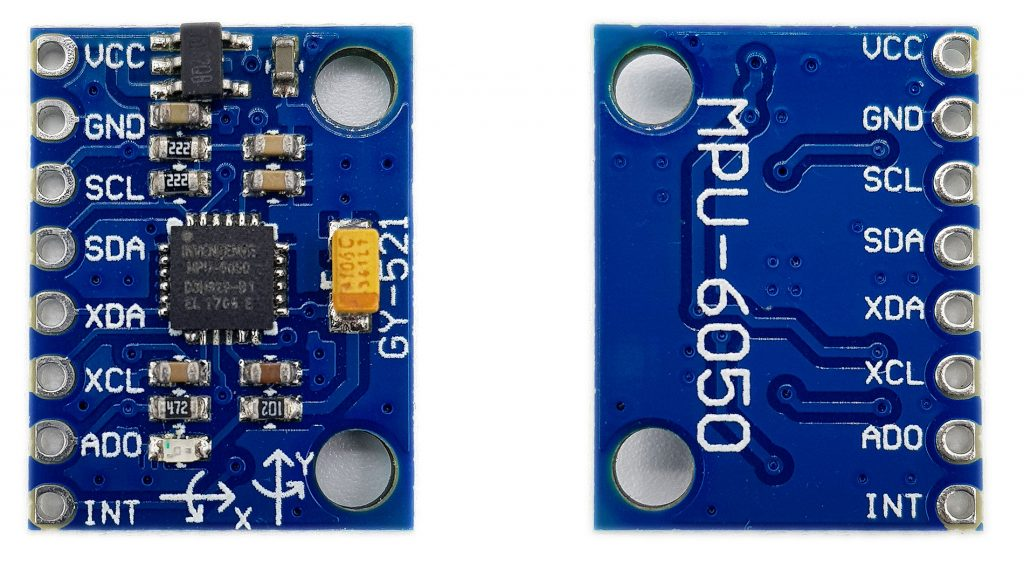
\includegraphics[width=0.7\linewidth]{images/Modul.jpg}
	\caption[Modul]{Modul}
	\label{fig:Modul}
\end{figure}

\cite{MPU6050}

\subsection{Trägheitsnavigation}

Die Trägheitsnavigation nutzt die physikalische Eigenschaften der Trägheit, um fortlaufende Berechnung der Position, Orientierung und Geschwindigkeit eines Objekts zu ermöglichen. Es ist immer nur die Anfangsposition bekannt, anhand dieser wird die spätere Position eines Objektes errechnet. Auch in GPS-gestörten Umgebungen z.B. Gebäuden, funktioniert die Trägheitsnavigation. 

\cite{Traegheitsnavigation}


\section{Software}


\subsection{Mobil Apps Grundlagen}

\textbf{Native Apps}

Native Apps (\emph{=deu.: angepasste Anwendung}) sind Anwendungen, die speziell für ein Betriebssystem (Android, iOS) entwickelt wurden. 

\cite{NativeApps}


\textbf{Android}


\textbf{iOS}

\subsection{Cross-Platform-Apps}

\textbf{Flutter}

Flutter ist eine Open-Source-Software, welche von Google entwickelt worden ist. Der Vorteil dieses Frameworks ist, dass man mit einem Programmcode in Flutter mehreren Apps auf verschiedenen Plattformen (Android, iOS) erstellen kann. Die Hauptprogrammiersprache ist Dart.

\cite{Flutter}

\textbf{React Native}

React Native ist eine Open-Source-Software, welche von Facebook entwickelt worden ist. Es wurde entwickelt, um Entwicklern mit Erfahrungen in React die Möglichkeit zu geben, einfacher Android Apps basierend auf React zu entwicklen. Die Hauptprogrammiersprachen sind JavaScript oder TypeScript.

\cite{React Native}





\chapter{Ergebnisdokumentation}
\textbf{TBD}


